\documentclass[12pt,a4paper]{article}
\usepackage[utf8]{inputenc}
\usepackage[T1]{fontenc}
\usepackage{lmodern} % Font standard di LaTeX (Computer Modern), come nel nuovo documento
\usepackage{graphicx}
\usepackage{geometry}
\geometry{a4paper, top=3cm, bottom=3cm, left=2.5cm, right=2.5cm}
\usepackage{xcolor}
\usepackage{hyperref}
\usepackage{parskip}
\usepackage{float}
\usepackage{listings}

\definecolor{unipiblue}{RGB}{0,51,102}

\hypersetup{
    colorlinks=true,
    linkcolor=black,
    filecolor=magenta,      
    urlcolor=blue,
    pdftitle={Distributed Crazy Time},
}

\begin{document}

% --- TITLE PAGE ---
\begin{titlepage}
    \begin{center}
        \vspace*{0.5cm}
        
        \IfFileExists{unipi_logo.png}{
\includegraphics[width=0.35\textwidth]{unipi_logo.png}}{\rule{4cm}{4cm}} \\
        \vspace{1cm}
        
        {\fontsize{34}{40}\selectfont \textcolor{unipiblue}{\scshape Università di Pisa}} \\
        \vspace{0.6cm}
        {\Large Computer Engineering} \\
        {\Large Distributed Systems} \\
        
        \vspace{3.5cm}
        
        {\huge \textbf{Distributed Crazy Time}} \\
        
        \vfill
        
        \noindent\rule{\textwidth}{0.4pt} \\
        \vspace{0.5cm}
        \begin{minipage}[t]{0.45\textwidth}
            \begin{flushleft}
            \vspace{0.8cm}
            Academic Year: 2025/2026
            \end{flushleft}
        \end{minipage}
        \hfill
        \begin{minipage}[t]{0.45\textwidth}
            \begin{flushright}
            Gabriele Caioli \\
            Klaudio Ciacia \\
            Lorenzo Vanni
            \end{flushright}
        \end{minipage}
        \vspace{1cm}
    \end{center}
\end{titlepage}

\tableofcontents
\newpage

\section{Introduction}
This project consists of a replica of the casino game Crazy Time, implemented as a web based application with three main layers:
\begin{itemize}
    \item A Web Layer (Frontend in HTML/CSS/JS and a Gateway implemented in Java Spring Boot) responsible for user management, wallets, and HTTP API serving.
    \item A Message Broker Layer using RabbitMQ for asynchronous communication between the Gateway and the Game Engine.
    \item A Distributed Game Engine implemented as a cluster of Erlang nodes, responsible for managing the state of the game, fair random number generation, executing the main wheel spins, and handling the interactions of the 4 asynchronous mini-games.
\end{itemize}
This architecture allows the system to guarantee real-time responsiveness and strong fault tolerance.

\begin{figure}[H]
    \centering
    \IfFileExists{wheel.png}{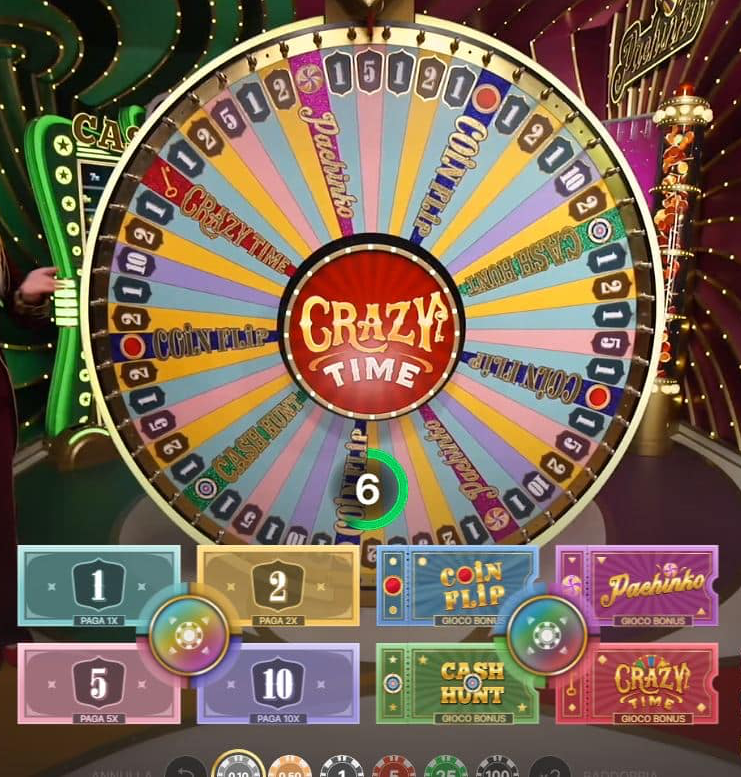
\includegraphics[width=0.7\textwidth]{wheel.png}}{\rule{0.7\textwidth}{5cm}}
\end{figure}

\subsection{Environment}
The Java-based part of the system (the gateway) has been implemented using Spring Boot, interacting with a local database for persistence. The Erlang-based components (the game engine cluster) have been developed using Erlang/OTP, utilizing Mnesia as a replicated distributed database to store the state. The communication middleware relies on RabbitMQ (AMQP Protocol).

\section{System Description}
The system is a web-based application providing functionalities for both account and wallet management, and real-time gameplay. The main supported operations include user registration, checking the wallet balance, placing bets on the main wheel or mini-games segments, and interacting during the mini-games phases.

\subsection{Use Cases}
An Unregistered User can:
\begin{itemize}
    \item Register to the service to create a wallet.
\end{itemize}
An Unlogged User can:
\begin{itemize}
    \item Login to the service as a Player.
\end{itemize}
A Logged Player can:
\begin{itemize}
    \item Logout;
    \item View the live countdown timer and the current state of the wheel/mini-games;
    \item Place bets on one or more wheel segments (if the betting window is open);
    \item View their current wallet balance and betting history.
\end{itemize}
The System must:
\begin{itemize}
    \item Maintain and update the Players' wallet balances securely;
    \item Synchronize the countdown timer and game status across all connected clients;
    \item Reject any bets placed after the "No more bets" signal;
    \item Generate a single, authoritative random outcome for each wheel spin and mini-game event;
    \item Gracefully recover from the crash of the node generating the game outcomes, ensuring the game continues without state corruption.
\end{itemize}

\subsection{The game}
Crazy Time is a live casino game with the following phases in each round:
\begin{enumerate}
    \item Betting: the user can bet some amount of money on any outcome of the wheel spin (numbers or minigames). This lasts until a timer expires.
    \item Lock: the bets are locked in and no more bets are accepted.
    \item Spin: the wheel spins and an outcome is decided based on the result
    \item Resolution: if the wheel lands on a number space, players who bet on that number receive a payout of the original bet multiplied by the number; if the wheel lands on a minigame space an interactive minigame starts for players who bet on that space; the bets on the space the wheel lands on are refunded and the other ones are lost
    \item Minigame (optional): if the wheel lands on a minigame space, the minigame starts; there are four possible minigames, two of which have an interactive element (crazy time and cash hunt) and two that do not (pachinko and coin flip)
\end{enumerate}

Clients do not communicate directly with Erlang; they communicate with the Java Gateway. The Java Gateway translates HTTP requests into AMQP messages.
\begin{itemize}
    \item Betting: Users place bets via /api/wallet/place-bet. The backend verifies the balance and issues a message to RabbitMQ.
    \item Mini-game interaction: During mini-games, users submit their choices (e.g., choosing a specific arrow in CrazyTime) to the Java API, which forwards them to the engine.
\end{itemize}

\subsubsection{Minigames}
There are four possible minigames that can start after a wheel spin:
\begin{itemize}
    \item Coin flip: two random multipliers are chosen and assigned to the two sides of a coin, then the coin is flipped and the players who bet on the minigame receive a payout of their bet multiplied by the multiplier decided by the outcome of the flip
    \item Pachinko: a pachinko machine appears and random multipliers are chosen for the bottom slots the ball could land in, then a ball is dropped in the machine from the top in a random spot and players receive a payot of their bet multiplied by the number the ball landed on
    \item Cash hunt: a grid of 108 multipliers is shown to the players, then each one is quickly covered by a random symbol from a set of 24 and shuffled around the board; players have a set amount of time to choose a spot on the board; the multipliers are revealed and each player gets a payout of their bet multiplies by the number under the symbol they chose
    \item Crazy time: a second wheel appears, with three arrows at the top instead of one and various multipliers on the spaces, players have time to choose one of the selectors before the spin, then the wheel spins and each player gets a payout of their bet multiplied by the number that landed on the arrow they chose
\end{itemize}

\subsection{Architecture}
The architecture is designed to decouple the client-facing APIs from the authoritative game logic, using a message queue.

\begin{figure}[H]
    \centering
    \IfFileExists{architecture.png}{
\includegraphics[width=\textwidth]{architecture.png}}{\rule{\textwidth}{6cm}}
\end{figure}

\subsubsection{Central node (Java Gateway)}
The central node is implemented using the Spring Boot framework. It provides the REST APIs for user registration, wallet management, and placing bets. It is the only component that interacts directly with the relational database holding user accounts and balances. When a bet is placed, the Gateway deducts the balance locally and forwards a structured JSON message containing a unique bet\_id via RabbitMQ to the Erlang Engine. It also listens to specific queues to process payouts or refunds sent back by the engine.

\subsubsection{Message Broker (RabbitMQ)}
Native AMQP integration allows full decoupling. The Gateway produces to a bets\_queue consumed by the Erlang cluster, and listens to queues for state updates (state\_queue), game results (results\_queue), and refunds (refunds\_queue).

\subsubsection{Game Server Cluster (Erlang Engine)}
The Erlang game engine runs on a cluster of nodes (typically 3). The game server acts authoritatively: it decides when the betting window closes, calculates the global ledger of accepted bets, spins the wheel, and resolves the outcomes. The nodes discover each other and form a highly available cluster.

\begin{figure}[H]
    \centering
    \IfFileExists{nodes.png}{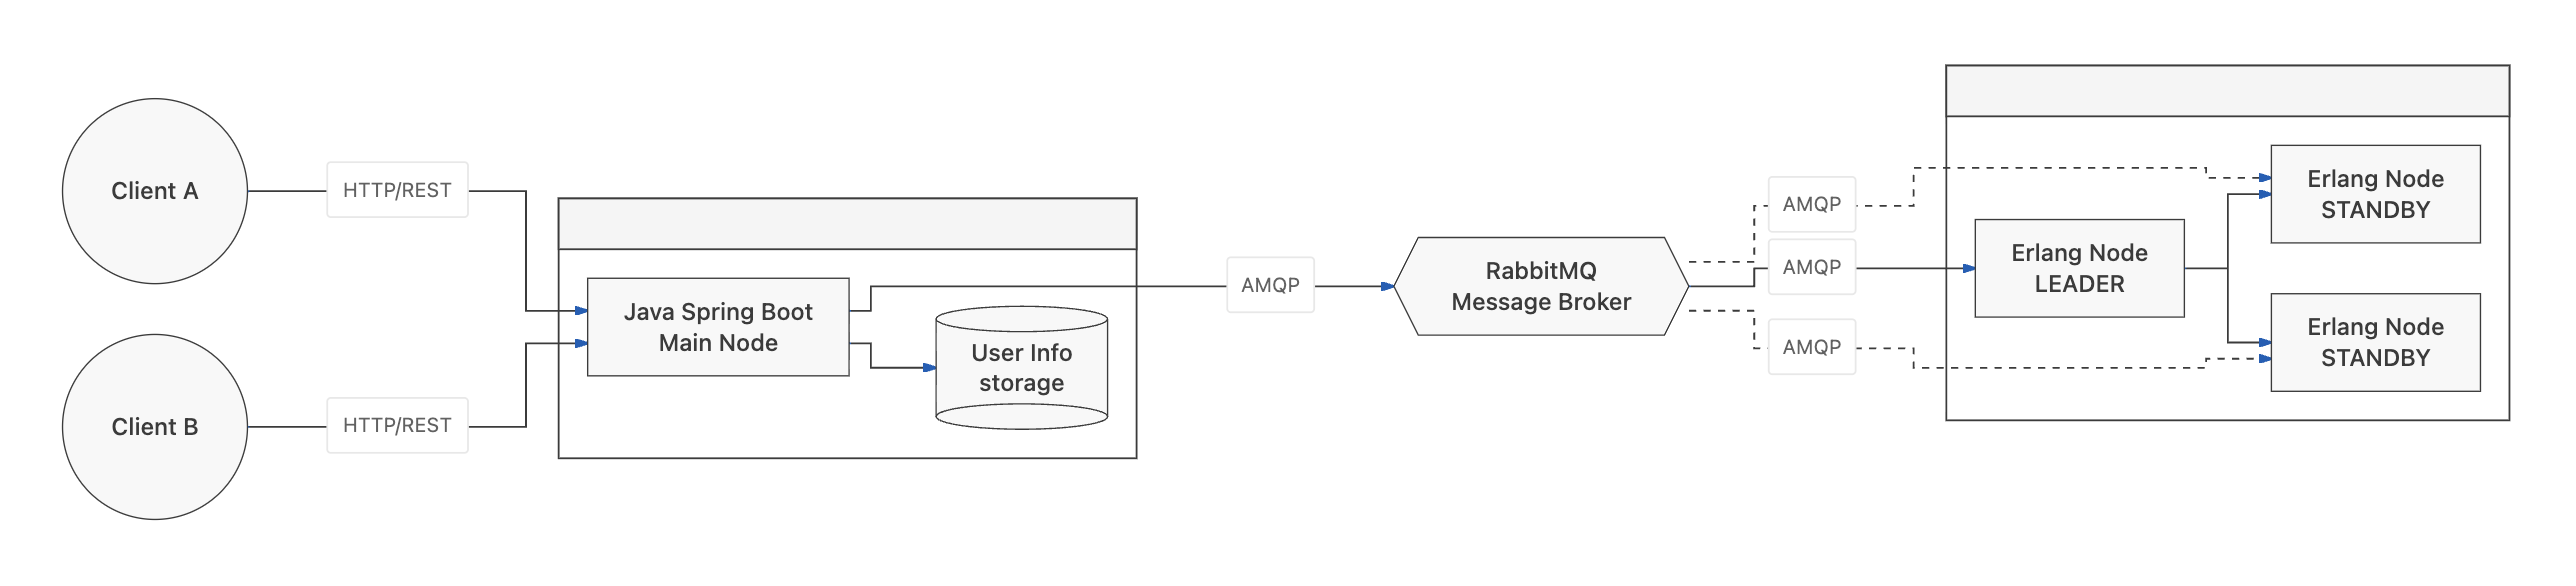
\includegraphics[width=0.8\textwidth]{nodes.png}}{\rule{0.8\textwidth}{5cm}}
\end{figure}

\subsection{Dealer Election}
The Erlang game engine runs on multiple nodes at once, if they all processed the game independently they would all spin their own wheel and pay out winnings to customers, who might even received duplicated payouts. To solve this issue a Dealer (Leader) node is elected, and it will be the only one who spins the wheel and calculates payouts. The election is done using the Bully algorithm:
\begin{enumerate}
    \item Each node has a unique identifier (e.g., game1, game2, game3).
    \item The node with the highest ID always wins the election and acts as the Leader.
    \item The other nodes act in a Standby role, simply forwarding incoming bets to the Leader.
    \item The system requires a Quorum (majority of nodes) to operate, preventing Split-Brain scenarios in case of network partitions.
    \item If the current Leader crashes, the remaining nodes detect the failure and immediately hold a new election. The highest ID among the survivors becomes the new Leader.
\end{enumerate}

\subsection{Synchronization}

\subsubsection{Snapshots}
Users playing the game only have a certain amount of time to place bets, after which bets are locked in and the game starts for everyone, so the system needs to know which bets were made in time and which were made too late and need to be rejected. Since Erlang processes and AMQP queues operate asynchronously, the \textbf{Chandy-Lamport Snapshot Algorithm} has been implemented to avoid race conditions and decide accurately the cutoff point for valid bets:
\begin{enumerate}
    \item Competing Consumers: Workers on all nodes consume bets from RabbitMQ asynchronously and forward them to the Leader's wheel\_process.
    \item The Marker: When the timer expires, the wheel\_process (Leader) saves its local state (received bets and extracted winner) and sends a "Snapshot Marker" backwards to all workers.
    \item In-Flight Messages: Workers receive the Marker, record their local state, and send a Marker back to the Leader.
    \item Capturing Channel State: Crucially, any bet that arrives at the Leader after the Leader started the snapshot, but before it receives the Marker back from the worker, was effectively "in-flight" across the network when the gong rang. These in-flight bets are causally part of the current round and are rightfully captured and included.
    \item The Ledger: A dedicated Collector process aggregates these local and channel states to form the authoritative Ledger of the round, which is saved to Mnesia as a Checkpoint.
\end{enumerate}

\subsubsection{State recovery}
If the Leader crashes after the betting phase but before the round ends, no bets are lost.
\begin{enumerate}
    \item A new Leader is elected via the Bully Algorithm.
    \item The new Leader reads the latest Checkpoint from Mnesia.
    \item The new Leader resumes the game, spins the wheel, calculates the outcomes based on the recovered ledger, and correctly issues payouts and refunds over RabbitMQ, ensuring zero financial loss for the players.
\end{enumerate}

\section{Implementation}

\subsection{Database Node}
The database is implemented using a MySQL server and it is responsible for keeping all users accounts and bets information.

\subsubsection{User table}
User is one of the tables implemented in the database. It contains the following columns:
\begin{itemize}
    \item username: username associated to the account.
    \item password: hashed password.
    \item balance: current wallet balance of the user.
\end{itemize}

\subsubsection{Bet table}
The Bet table tracks all wagers. It contains:
\begin{itemize}
    \item bet\_id: unique UUID for the bet.
    \item username: reference to the user.
    \item amount: wager amount.
    \item segment: the target segment of the wheel.
    \item status: PENDING, WON, LOST, REFUNDED.
    \item round: the round number it was placed in.
\end{itemize}

\subsection{Central Node (Java)}
The central node is the first point of contact for the clients with the distributed system. It consists in a Web Server implemented using the Springboot framework.

\subsubsection{Source code structure}
The source code is organized in the following packages:
\begin{itemize}
    \item config: contains classes for handling the configuration parameters of the security and web sockets.
    \item controller: Springboot controllers for mapping all endpoints.
    \item dto: classes used for instantiating the Data Transfer Objects.
    \item entity: classes for representing the database data.
    \item rabbitmq: classes where the AMQP logic and listeners are developed.
    \item repository: classes for the database interaction.
    \item security: classes for interception and validation of requests.
    \item service: classes with the business logic.
\end{itemize}

\subsubsection{The config package}
It contains classes like SecurityConfig and WebSocketConfig.
\begin{itemize}
    \item SecurityConfig: It defines Java Beans useful for the security aspects. The SecurityFilterChain bean defines a filter to be applied in incoming requests and protects endpoints.
    \item WebSocketConfig: Configures STOMP over WebSocket for real-time game updates.
\end{itemize}

\subsubsection{The controller package}
A total of 3 controllers are used.
\begin{itemize}
    \item AuthController: Provides endpoints used for handling login and registration.
    \item WalletController: Provides REST API endpoints for requests relative to money and bets:
    \begin{itemize}
        \item POST /api/wallet/place-bet: validates user balances, creates a unique bet\_id, uses pessimistic locking (@Lock(LockModeType.\allowbreak PESSIMISTIC\_WRITE)) on the database to prevent double-spending, and forwards the payload to RabbitMQ.
    \end{itemize}
    \item GameController: Handles interactions during the mini-games (e.g., submitting a choice for CashHunt).
\end{itemize}

\subsubsection{The rabbitmq package}
Crucial for the asynchronous integration with the Game Engine.
\begin{itemize}
    \item PayoutListener: Listens to the results\_queue AMQP queue. When a round finishes, it securely credits winning bets to user wallets. It ensures idempotency by verifying the bet status, thus avoiding duplicate payouts.
    \item RefundListener: Listens to the refunds\_queue. If the Erlang engine rejects a bet, this listener restores the deducted balance.
    \item GameStateCache: An atomic cache holding the most recent state broadcasted by the engine.
\end{itemize}

\subsection{Erlang Game Engine}
The Game Engine is designed to handle the core game logic and runs on a distributed Erlang cluster.

\subsubsection{Source code structure}
The following files are defined in the src/ directory:
\begin{itemize}
    \item game\_engine\_app.src --- configuration file of the application.
    \item game\_engine\_app.erl --- application entry point.
    \item game\_engine\_sup.erl --- node supervisor.
    \item cluster\_manager.erl --- manages the distributed cluster state.
    \item leader\_election.erl --- implements the Bully Algorithm.
    \item rabbitmq\_manager.erl \& worker.erl --- AMQP handlers.
    \item wheel\_process.erl --- core game logic implemented via gen\_server.
    \item cl\_recorder.erl \& snapshot.erl --- Chandy-Lamport snapshot algorithm.
    \item minigames\_sup.erl and mini-games modules (pachinko.erl, cashhunt.erl, etc.).
\end{itemize}

\subsubsection{Fault Tolerance Modules}
\begin{itemize}
    \item leader\_election.erl: Implements the fault-tolerance mechanism. It runs periodically, sending heartbeats to peer nodes. If it detects that the highest-ID node is dead, it promotes its own node if it holds the highest surviving ID, taking over the wheel\_process duties.
    \item cluster\_manager.erl: Maintains the lists of active nodes and configured nodes to evaluate quorums and avoid split-brain scenarios.
\end{itemize}

\subsubsection{Core Game Modules}
\begin{itemize}
    \item wheel\_process.erl:
    \begin{itemize}
        \item Behaviour: gen\_server.
        \item Responsibilities: This process manages the timer lifecycle. When the betting phase ends, it coordinates with the snapshot modules to lock the bets. Then, it calculates the winning segment. If the segment is a number, it computes payouts. If it's a mini-game, it delegates the execution to the specific mini-game module.
    \end{itemize}
    \item worker.erl: Dedicated processes that consume AMQP messages from bets\_queue. In a Standby node, a worker simply routes the bet to the Leader node via standard Erlang Distribution (!). In the Leader node, the worker passes the bet to the local wheel\_process.
    \item cl\_recorder.erl: A pure functional module that records the local state of a worker when the "Snapshot Marker" is received, essential to build the globally consistent Checkpoint stored in Mnesia.
\end{itemize}

\subsubsection{Mini-games}
The mini-games are spawned as separate processes under minigames\_sup.erl. For example, cashhunt.erl initializes a 9x12 grid of 108 hidden multipliers using a realistic probability distribution. It waits for choices routed from the Java Gateway and finally computes the exact payout for each participating user.

\section{Demonstration}

\subsection{Run the system}
To launch the project, you need multiple terminals. The startup sequence is as follows:

1. Start RabbitMQ (Terminal 1) Navigate to the RabbitMQ installation folder and start the server:

\begin{lstlisting}[basicstyle=\ttfamily, breaklines=true]
cd "C:\Program Files\RabbitMQ Server\rabbitmq_server-4.3.4\sbin"
.\rabbitmq-server.bat
\end{lstlisting}
(Management interface available at \url{http://localhost:15672})

2. Start Java Gateway (Terminal 2) Navigate to the java-gateway folder and run the Spring Boot application:

\begin{lstlisting}[basicstyle=\ttfamily, breaklines=true]
cd java-gateway
mvn spring-boot:run
\end{lstlisting}

3. Start the Erlang Cluster (Terminals 3, 4, 5) Navigate to the Erlang game engine directory. You need to start 3 instances using the same cookie but different node names to form the cluster. (Note: Use rebar3 shell as erl direct calls might fail to expand paths on Windows)

Terminal 3 (Node 1):

\begin{lstlisting}[basicstyle=\ttfamily, breaklines=true]
cmd
cd erlang-engine\game_engine
set ERL_FLAGS=-sname game1@localhost -setcookie crazytime
escript ..\rebar3 shell
\end{lstlisting}

Terminal 4 (Node 2):

\begin{lstlisting}[basicstyle=\ttfamily, breaklines=true]
cd erlang-engine\game_engine
set ERL_FLAGS=-sname game2@localhost -setcookie crazytime
escript ..\rebar3 shell
\end{lstlisting}

Terminal 5 (Node 3 - Leader):

\begin{lstlisting}[basicstyle=\ttfamily, breaklines=true]
cd erlang-engine\game_engine
set ERL_FLAGS=-sname game3@localhost -setcookie crazytime
escript ..\rebar3 shell
\end{lstlisting}

Note for PowerShell users: set the environment variable using \texttt{\$env:ERL\_FLAGS = "-sname game1@localhost}\allowbreak \texttt{-setcookie crazytime"}.\\
Once the 3 nodes are up, the Bully Algorithm automatically elects game3 as the Leader (Dealer), while the other two become Standby nodes.

\subsection{Interaction}
You can interact with the system via the Web UI provided by the Java Gateway at \url{http://localhost:8080}, or via REST calls using curl:

\begin{lstlisting}[basicstyle=\ttfamily, breaklines=true]
# Register User
curl.exe -X POST 
"http://localhost:8080/api/wallet/register?username=testuser"

# Place Bet
curl.exe -X POST 
"http://localhost:8080/api/wallet/place-bet?username=testuser&amount=10.00&segment=5"
\end{lstlisting}

\end{document}
